\documentclass{article}

% if you need to pass options to natbib, use, e.g.:
% \PassOptionsToPackage{numbers, compress}{natbib}
% before loading nips_2016
%
% to avoid loading the natbib package, add option nonatbib:
% \usepackage[nonatbib]{nips_2016}

\usepackage[final]{nips_2016}

% FONTS
\usepackage[T1]{fontenc}
\usepackage{tgtermes}
\usepackage{amsmath}
\usepackage{enumitem}

% Font choice 1:
\usepackage[subscriptcorrection,
           amssymbols,
           mtpbb,
           mtpcal,
           nofontinfo  % suppresses all warnings
          ]{mtpro2}

% Font choice 2:
%\usepackage[scaled=0.92]{PTSans}
%\usepackage{amssymb}
%\newcommand{\mathbold}[1]{\ensuremath{\boldsymbol{\mathbf{#1}}}}
%\newcommand{\mbf}[1]{\ensuremath{\boldsymbol{\mathbf{#1}}}}
%\newcommand{\hmbtheta}{\mathbold{\widehat{\theta}}}
%\newcommand{\hb}{\mathbold{\widehat{b}}}
%\newcommand{\hB}{\mathbold{\widehat{B}}}
%\newcommand{\hbP}{\mathbold{\widehat{P}}}

\usepackage{scalefnt,letltxmacro}
\LetLtxMacro{\oldtextsc}{\textsc}
\renewcommand{\textsc}[1]{\oldtextsc{\scalefont{1.10}#1}}

% \renewcommand*\ttdefault{lmvtt}
\usepackage[ttdefault=true]{AnonymousPro}

% GEOMETRY
%\usepackage[
%  paper  = letterpaper,
%  left   = 1.65in,
%  right  = 1.65in,
%  top    = 1.0in,
%  bottom = 1.0in,
%  ]{geometry}

% COLOR
\usepackage[usenames,dvipsnames]{xcolor}
\definecolor{shadecolor}{gray}{0.9}

% SPACING and TEXT
%\usepackage[final,expansion=alltext]{microtype}
\usepackage[english]{babel}
\usepackage[parfill]{parskip}
\usepackage{afterpage}
\usepackage{framed}

%redefine the leftbar environment to accept a width and coloring options
\renewenvironment{leftbar}[1][\hsize]
{%
  \def\FrameCommand
  {%
    {\color{Gray}\vrule width 3pt}%
    \hspace{10pt}%
    %\hspace{0pt}\fboxsep=\FrameSep\colorbox{black!10}%
  }%
  \MakeFramed{\hsize#1\advance\hsize-\width\FrameRestore}%
}%
{\endMakeFramed}

% define a paragraph header function
\DeclareRobustCommand{\parhead}[1]{\textbf{#1}~}

% EDITING
% line numbering in left margin
\usepackage{lineno}
\renewcommand\linenumberfont{\normalfont

             \footnotesize
                             \sffamily
                             \color{SkyBlue}}
% ragged paragraphs in right margin
\usepackage{ragged2e}
\DeclareRobustCommand{\sidenote}[1]{\marginpar{
                                    \RaggedRight
                                    \textcolor{Plum}{\textsf{#1}}}}
% paragraph counter in right margin
\newcommand{\parnum}{\bfseries\P\arabic{parcount}}
\newcounter{parcount}
\newcommand\p{%
    \stepcounter{parcount}%
    \leavevmode\marginpar[\hfill\parnum]{\parnum}%
}
% paragraph helper
\DeclareRobustCommand{\PP}{\textcolor{Plum}{\P} }

% COUNTERS
\renewcommand{\labelenumi}{\color{black!67}{\arabic{enumi}.}}
\renewcommand{\labelenumii}{{\color{black!67}(\alph{enumii})}}
\renewcommand{\labelitemi}{{\color{black!67}\textbullet}}

% FIGURES
\usepackage{graphicx}
\usepackage[labelfont=bf]{caption}
\usepackage[format=hang]{subcaption}

% TABLES
\usepackage{booktabs}

% ALGORITHMS
\usepackage[algoruled]{algorithm2e}
\usepackage{listings}
\usepackage{fancyvrb}
\fvset{fontsize=\normalsize}

% BIBLIOGRAPHY
\usepackage[numbers]{natbib}

% HYPERREF
\usepackage[colorlinks,linktoc=all]{hyperref}
%\usepackage[all]{hypcap}
\hypersetup{citecolor=Blue}
\hypersetup{linkcolor=MidnightBlue}
\hypersetup{urlcolor=MidnightBlue}

% ##### CLEVERREF
\usepackage[nameinlink]{cleveref}
\creflabelformat{equation}{#1#2#3}

% CLEVEREF alternative
\newcommand{\myeqp}[1]{Eq.\ref{eq:#1}}
\newcommand{\mysec}[1]{Section~\ref{sec:#1}}
\newcommand{\mytable}[1]{Table~\ref{table:#1}}
\newcommand{\myfig}[1]{Figure~\ref{fig:#1}}
\newcommand{\myappendix}[1]{Appendix \ref{appendix:#1}}
\newcommand{\myalg}[1]{Algorithm~\ref{alg:#1}}

% ACRONYMS
\usepackage
[acronym,smallcaps,nowarn,section,nogroupskip,nonumberlist]{glossaries}
\glsdisablehyper{}
% \makeglossaries

% COLOR DEFINITIONS
\newcommand{\red}[1]{\textcolor{BrickRed}{#1}}
\newcommand{\orange}[1]{o\textcolor{BurntOrange}{#1}}
\newcommand{\green}[1]{\textcolor{OliveGreen}{#1}}
\newcommand{\blue}[1]{\textcolor{MidnightBlue}{#1}}
\newcommand{\gray}[1]{\textcolor{black!60}{#1}}

% LISTINGS DEFINTIONS
\lstdefinestyle{mystyle}{
    commentstyle=\color{OliveGreen},
    keywordstyle=\color{BurntOrange},
    numberstyle=\tiny\color{black!60},
    stringstyle=\color{MidnightBlue},
    basicstyle=\ttfamily,
    breakatwhitespace=false,
    breaklines=true,
    captionpos=b,
    keepspaces=true,
    numbers=left,
    numbersep=5pt,
    showspaces=false,
    showstringspaces=false,
    showtabs=false,
    tabsize=2
}
\lstset{style=mystyle}

%\usepackage{titlesec}
%\titlespacing*{\section}{0pt}{1.1\baselineskop}{\baselineskip}

% A
\newacronym{ADVI}{advi}{automatic differentiation variational inference}

% B
\newacronym{BBVI}{bbvi}{black-box variational inference}

% C
\newacronym{CTM}{ctm}{correlated topic model}

% D
\newacronym[\glslongpluralkey={deep exponential families}]{DEF}{def}{deep exponential family}
\newacronym{DMIS}{dmis}{deterministic multiple importance sampling}

% E
\newacronym{ELBO}{elbo}{evidence lower bound}

% G
\newacronym{GNTS}{gn-ts}{gamma-normal time series model}
\newacronym{G-REP}{g-rep}{generalized reparameterization}

% K
\newacronym{KL}{kl}{{K}ullback-{L}eibler}

% L
\newacronym{LDA}{lda}{latent {D}irichlet allocation}

% M
\newacronym{MF}{mf}{matrix factorization}
\newacronym{MIS}{mis}{multiple importance sampling}
\newacronym{MATLAB}{matlab}{MATLAB}

\newacronym{NIPS}{nips}{Neural Information Processing Systems}

% O
\newacronym{OBBVI}{o-bbvi}{overdispersed black-box variational inference}

% R
\newacronym{RS-VI}{rsvi}{rejection sampling variational inference}

% S
\newacronym{SVI}{svi}{stochastic variational inference}

% V
\newacronym{VI}{vi}{variational inference}


% !TEX root = main.tex

% project specific

%\newcommand{\mbx}{\textbf{x}}
%\newcommand{\mbrho}{\mb{\rho}}
%\newcommand{\mbalpha}{\mb{\alpha}}
\newcommand{\expfam}{\textrm{ExpFam}}


% \DeclareRobustCommand{\mb}[1]{\ensuremath{\boldsymbol{\mathbf{#1}}}}
\DeclareRobustCommand{\mb}[1]{\mathbold{#1}}

\DeclareRobustCommand{\KL}[2]{\ensuremath{\textrm{KL}\left(#1\;\|\;#2\right)}}

\DeclareMathOperator*{\argmax}{arg\,max}
\DeclareMathOperator*{\argmin}{arg\,min}

\renewcommand{\mid}{~\vert~}
\newcommand{\prm}{\:;\:}

\newcommand{\mbw}{\mb{w}}
\newcommand{\mbW}{\mb{W}}

\newcommand{\mbx}{\mb{x}}
\newcommand{\mbX}{\mbf{X}}

\newcommand{\mby}{\mb{y}}
\newcommand{\mbY}{\mbf{Y}}

\newcommand{\mbz}{\mb{z}}
\newcommand{\mbZ}{\mb{Z}}

\newcommand{\mbI}{\mbf{I}}
\newcommand{\mbone}{\mbf{1}}

\newcommand{\mbL}{\mbf{L}}

\newcommand{\mbtheta}{\mb{\theta}}
\newcommand{\mbTheta}{\mb{\Theta}}
\newcommand{\mbomega}{\mb{\omega}}
\newcommand{\mbOmega}{\mb{\Omega}}
\newcommand{\mbsigma}{\mb{\sigma}}
\newcommand{\mbSigma}{\mb{\Sigma}}
\newcommand{\mbphi}{\mb{\phi}}
\newcommand{\mbPhi}{\mb{\Phi}}

\newcommand{\mbalpha}{\mb{\alpha}}
\newcommand{\mbbeta}{\mb{\beta}}
\newcommand{\mbgamma}{\mb{\gamma}}
\newcommand{\mbeta}{\mb{\eta}}
\newcommand{\mbmu}{\mb{\mu}}
\newcommand{\mbrho}{\mb{\rho}}
\newcommand{\mblambda}{\mb{\lambda}}
\newcommand{\mbzeta}{\mb{\zeta}}

\newcommand\dif{\mathop{}\!\mathrm{d}}
\newcommand{\diag}{\textrm{diag}}
\newcommand{\supp}{\textrm{supp}}

\newcommand{\E}{\mathbb{E}}
\newcommand{\V}{\mathbb{V}}
\newcommand{\bbH}{\mathbb{H}}

\newcommand{\bbN}{\mathbb{N}}
\newcommand{\bbZ}{\mathbb{Z}}
\newcommand{\bbR}{\mathbb{R}}
\newcommand{\bbS}{\mathbb{S}}

\newcommand{\cL}{\mathcal{L}}

\newcommand{\cN}{\mathcal{N}}
\newcommand{\cT}{\mathcal{T}}
\newcommand{\Gam}{\textrm{Gam}}
\newcommand{\InvGam}{\textrm{InvGam}}

\newcommand{\g}{\, | \,}


% to compile a camera-ready version, add the [final] option, e.g.:
% \usepackage[final]{nips_2016}

\title{The Generalized Reparameterization Gradient:\\Supplement}

% The \author macro works with any number of authors. There are two
% commands used to separate the names and addresses of multiple
% authors: \And and \AND.
%
% Using \And between authors leaves it to LaTeX to determine where to
% break the lines. Using \AND forces a line break at that point. So,
% if LaTeX puts 3 of 4 authors names on the first line, and the last
% on the second line, try using \AND instead of \And before the third
% author name.

\author{
  Francisco J.~R.~Ruiz\\
  University of Cambridge\\
  Columbia University\\
  \And
  Michalis K.~Titsias\\
  Athens University of\\Economics and Business\\
  \And
  David M.~Blei\\
  Columbia University\\
}

\begin{document}

\maketitle

%%%%%%%%%%%%%%%%%%%%%%%%%%%%%%%%%%%%%%%%%%%%%%%%%%%%%%%%%%%%%%%%%
\section{Derivation of the Generalized Reparameterization Gradient}

Here we show the mathematical derivation of the generalized reparameterization gradient. Firstly, recall the definition of the functions 
\begin{align}
    & \hfun(\beps;\bv)\triangleq \nabla_{\bv} \Tcal(\beps;\bv), \\
    & \ufun(\beps;\bv)\triangleq \nabla_{\bv} \log J(\beps,\bv),
\end{align}
which are provided in the main text.

We start from the following expression of the gradient, also derived in the main text:
\begin{equation}
    \nabla_{\bv} \E{q(\bz;\bv)}{f(\bz)} = \underbrace{\int q_{\beps}(\beps;\bv)\nabla_{\bv}f\left(\Tcal(\beps;\bv)\right)d\beps}_{\bg^{\textrm{rep}}} +
    \underbrace{\int q_{\beps}(\beps;\bv)f\left(\Tcal(\beps;\bv)\right)\nabla_{\bv} \log q_{\beps}(\beps;\bv) d\beps}_{\bg^{\textrm{corr}}},
\end{equation}

We can write the former term, $\bg^{\textrm{rep}}$, as
\begin{align}
    \bg^{\textrm{rep}} & = \int q_{\beps}(\beps;\bv)\nabla_{\bv}f\left(\Tcal(\beps;\bv)\right)d\beps \\ 
    & = \int q\left(\Tcal(\beps;\bv);\bv\right)J(\beps,\bv) \nabla_{\bv}f\left(\Tcal(\beps;\bv)\right)d\beps \\
    & = \int q\left(\Tcal(\beps;\bv);\bv\right)J(\beps,\bv) \nabla_{\bz}f(\bz)\big|_{\bz=\Tcal(\beps;\bv)} \nabla_{\bv} \Tcal(\beps;\bv)d\beps \\
    & = \int q(\bz;\bv) \nabla_{\bz}f(\bz) \hfun\left( \Tcal^{-1}(\bz;\bv);\bv \right) d\bz \\
    & = \E{q(\bz;\bv)}{\nabla_{\bz}f(\bz) \hfun\left( \Tcal^{-1}(\bz;\bv);\bv \right)},
\end{align}
where we have first replaced the variational distribution on the transformed space with its form as a function of $q(\bz;\bv)$, i.e., $q_{\beps}(\beps;\bv) = q\left(\Tcal(\beps;\bv);\bv\right)J(\beps,\bv)$. We have then applied the chain rule, and finally we have made a new change of variables back to the original space $\bz$ (thus multiplying by the inverse Jacobian).

For the latter, $\bg^{\textrm{corr}}$, we have that
\begin{align}
    \bg^{\textrm{corr}} & = \int q_{\beps}(\beps;\bv)f\left(\Tcal(\beps;\bv)\right)\nabla_{\bv} \log q_{\beps}(\beps;\bv) d\beps \\ 
    & = \int q\left(\Tcal(\beps,\bv);\bv\right)J(\beps,\bv)f\left(\Tcal(\beps;\bv)\right)\nabla_{\bv} \left(\log q\left(\Tcal(\beps;\bv);\bv\right)+\log J(\beps,\bv)\right) d\beps \\ 
    & = \int q\left(\Tcal(\beps;\bv);\bv\right)J(\beps,\bv)f\left(\Tcal(\beps;\bv)\right)\left( \nabla_{\bv} \log q\left(\Tcal(\beps;\bv);\bv\right)+\nabla_{\bv} \log J(\beps,\bv)\right) d\beps. 
\end{align}
The derivative $\nabla_{\bv}\log q\left(\Tcal(\beps;\bv);\bv\right)$ can be obtained by the chain rule. If $\bz=\Tcal(\beps;\bv)$, then $\nabla_{\bv}\log q\left(\Tcal(\beps;\bv);\bv\right)=\nabla_{\bz}\log q(\bz;\bv) \nabla_{\bv}\Tcal(\beps;\bv) + \nabla_{\bv}\log q(\bz;\bv)$. We substitute this result in the above equation and revert the change of variables back to the original space $\bz$ (also multiplying by the inverse Jacobian), yielding
\begin{equation}\label{eq:g_corr}
  \begin{split}
    \bg^{\textrm{corr}} & = \int q(\bz;\bv) f(\bz) \left(\nabla_{\bz}\log q(\bz;\bv) \hfun\left(\Tcal^{-1}(\bz;\bv);\bv\right) + \nabla_{\bv}\log q(\bz;\bv)+ \ufun\left(\Tcal^{-1}(\bz;\bv);\bv \right) \right) d\bz \\
    & = \E{q(\bz;\bv)}{f(\bz) \left(\nabla_{\bz}\log q(\bz;\bv) \hfun\left(\Tcal^{-1}(\bz;\bv);\bv\right) + \nabla_{\bv}\log q(\bz;\bv)+ \ufun\left(\Tcal^{-1}(\bz;\bv);\bv \right) \right)},
  \end{split}
\end{equation}
where we have used the definition of the functions $\hfun(\beps;\bv)$ and $\ufun(\beps;\bv)$.

\section{Particularization for the Gamma Distribution}

For the gamma distribution we choose the transformation
\begin{align}
z=\Tcal(\epsilon;\alpha,\beta)=\exp(\epsilon\sqrt{\psi_1(\alpha)}+\psi(\alpha)-\log(\beta)).
\end{align}
Thus, we have that
\begin{align}
    & J(\epsilon,\alpha,\beta) = |\det \nabla_{\epsilon}\Tcal(\epsilon;\alpha,\beta)| = \Tcal(\epsilon;\alpha,\beta)\sqrt{\psi_1(\alpha)}.
\end{align}
The derivatives of $\log q(z;\alpha,\beta)$ with respect to its arguments are given by
\begin{align}
    & \frac{\partial}{\partial z}\log q(z;\alpha,\beta) = \frac{\alpha-1}{z}-\beta,\\
    & \frac{\partial}{\partial \alpha}\log q(z;\alpha,\beta) = \log(\beta)-\psi(\alpha)+\log(z),\\
    & \frac{\partial}{\partial \beta}\log q(z;\alpha,\beta) = \frac{\alpha}{\beta}-z.
\end{align}

Therefore, the auxiliary functions $\hfun(\epsilon;\alpha,\beta)$ and $\ufun(\epsilon;\alpha,\beta)$ for the components of the gradient with respect to $\alpha$ and $\beta$ can be written as
\begin{align}
    & \hfun_{\alpha}(\epsilon;\alpha,\beta) = \frac{\partial}{\partial\alpha}\Tcal(\epsilon;\alpha,\beta) = \Tcal(\epsilon;\alpha,\beta) \left( \frac{\epsilon\psi_2(\alpha)}{2\sqrt{\psi_1(\alpha)}}+\psi_1(\alpha)\right),\\
    & \hfun_{\beta}(\epsilon;\alpha,\beta) = \frac{\partial}{\partial\beta}\Tcal(\epsilon;\alpha,\beta) = -\frac{\Tcal(\epsilon;\alpha,\beta)}{\beta},\\
    & \ufun_{\alpha}(\epsilon;\alpha,\beta) = \frac{\partial}{\partial\alpha}\log J(\epsilon,\alpha,\beta) = \left( \frac{\epsilon\psi_2(\alpha)}{2\sqrt{\psi_1(\alpha)}}+\psi_1(\alpha)\right)+\frac{\psi_2(\alpha)}{2\psi_1(\alpha)},\\
    & \ufun_{\beta}(\epsilon;\alpha,\beta) = \frac{\partial}{\partial\beta}\log J(\epsilon,\alpha,\beta) = -\frac{1}{\beta}.
\end{align}

Thus, we finally obtain that the components of $\bg^{\textrm{rep}}$ corresponding to the derivatives with respect to $\alpha$ and $\beta$ are given by
\begin{align}
    & \bg^{\textrm{rep}}_{\alpha} = \E{q(z;\alpha,\beta)}{\frac{\partial}{\partial z}f(\bz) \times z \left( \frac{\Tcal^{-1}(z;\alpha,\beta)\psi_2(\alpha)}{2\sqrt{\psi_1(\alpha)}}+\psi_1(\alpha)\right)},\\
    & \bg^{\textrm{rep}}_{\beta} = \E{q(z;\alpha,\beta)}{\frac{\partial}{\partial z}f(\bz) \times \frac{-z}{\beta}},
\end{align}
while the components of $\bg^{\textrm{corr}}$ can be similarly obtained by substituting the expressions above into Eq.~\ref{eq:g_corr}. Remarkably, we obtain that 
\begin{align}
    & \bg^{\textrm{corr}}_{\beta} = 0.
\end{align}

\section{Particularization for the Beta Distribution}

For a random variable $z\sim\textrm{Beta}(\alpha,\beta)$, we could rewrite $z=z_1^\prime/(z_1^\prime+z_2^\prime)$ for $z_1^\prime\sim\textrm{Gamma}(\alpha,1)$ and $z_2^\prime\sim\textrm{Gamma}(\beta,1)$, and apply the above method for the gamma-distributed variables $z_1^\prime$ and $z_2^\prime$. Instead, in the spirit of applying standardization directly over $z$, we define a transformation to standardize the logit function. This leads to
\begin{align}
    z=\Tcal(\epsilon;\alpha,\beta)=\frac{1}{1+\exp(-\epsilon\sigma-\psi(\alpha)+\psi(\beta))}.
\end{align}
This transformation ensures that $\epsilon$ has mean zero. However, in this case we do not specify the form of $\sigma$, and we let it be a function of $\alpha$ and $\beta$. This allows us to choose $\sigma$ in such a way that $\bg^{\textrm{corr}}=\bzero$ for the sampled value of $z$, which we found to work well (even though this introduces some bias). For simplicity, we write $\sigma=\exp(\phi)$.

Thus, we have that
\begin{align}
    & J(\epsilon,\alpha,\beta) = |\det \nabla_{\epsilon}\Tcal(\epsilon;\alpha,\beta)| = \Tcal(\epsilon;\alpha,\beta)(1-\Tcal(\epsilon;\alpha,\beta))\sigma.
\end{align}
The derivatives of $\log q(z;\alpha,\beta)$ with respect to its arguments are given by
\begin{align}
    & \frac{\partial}{\partial z}\log q(z;\alpha,\beta) = \frac{\alpha-1}{z} - \frac{\beta-1}{1-z},\\
    & \frac{\partial}{\partial \alpha}\log q(z;\alpha,\beta) = \psi(\alpha+\beta)-\psi(\alpha)+\log(z),\\
    & \frac{\partial}{\partial \beta}\log q(z;\alpha,\beta) = \psi(\alpha+\beta)-\psi(\beta)+\log(1-z).
\end{align}

Therefore, the auxiliary functions $\hfun(\epsilon;\alpha,\beta)$ and $\ufun(\epsilon;\alpha,\beta)$ for the components of the gradient with respect to $\alpha$ and $\beta$ can be written as
\begin{align}
    & \hfun_{\alpha}(\epsilon;\alpha,\beta) = \frac{\partial}{\partial\alpha}\Tcal(\epsilon;\alpha,\beta) = \Tcal(\epsilon;\alpha,\beta)(1-\Tcal(\epsilon;\alpha,\beta))\left( \psi_1(\alpha) + \epsilon\sigma\frac{\partial\phi}{\partial\alpha} \right) ,\\
    & \hfun_{\beta}(\epsilon;\alpha,\beta) = \frac{\partial}{\partial\beta}\Tcal(\epsilon;\alpha,\beta) = \Tcal(\epsilon;\alpha,\beta)(1-\Tcal(\epsilon;\alpha,\beta))\left( -\psi_1(\beta) + \epsilon\sigma\frac{\partial\phi}{\partial\beta} \right),\\
    & \ufun_{\alpha}(\epsilon;\alpha,\beta) = \frac{\partial}{\partial\alpha}\log J(\epsilon,\alpha,\beta) = (1-2\Tcal(\epsilon;\alpha,\beta))\left( \psi_1(\alpha) + \epsilon\sigma\frac{\partial\phi}{\partial\alpha} \right)+\frac{\partial\phi}{\partial\alpha},\\
    & \ufun_{\beta}(\epsilon;\alpha,\beta) = \frac{\partial}{\partial\beta}\log J(\epsilon,\alpha,\beta) = (1-2\Tcal(\epsilon;\alpha,\beta))\left( -\psi_1(\beta) + \epsilon\sigma\frac{\partial\phi}{\partial\beta} \right)+\frac{\partial\phi}{\partial\beta}.
\end{align}
Note that the term $\epsilon\sigma$ above can be computed from $z$ without knowledge of the value of $\sigma$ as $\epsilon\sigma=\Tcal^{-1}(z;\alpha,\beta)\sigma = \frac{\logit{z}-\psi(\alpha)+\psi(\beta)}{\sigma}\sigma=\logit{z}-\psi(\alpha)+\psi(\beta)$.

Thus, we finally obtain that the components of $\bg^{\textrm{rep}}$ corresponding to the derivatives with respect to $\alpha$ and $\beta$ are given by
\begin{align}
    & \bg^{\textrm{rep}}_{\alpha} = \E{q(z;\alpha,\beta)}{\frac{\partial}{\partial z}f(\bz) \times z(1-z)\left( \psi_1(\alpha) + \left(\logit{z}-\psi(\alpha)+\psi(\beta)\right)\frac{\partial\phi}{\partial\alpha} \right)},\\
    & \bg^{\textrm{rep}}_{\beta} = \E{q(z;\alpha,\beta)}{\frac{\partial}{\partial z}f(\bz) \times z(1-z)\left( -\psi_1(\beta) + \left(\logit{z}-\psi(\alpha)+\psi(\beta)\right)\frac{\partial\phi}{\partial\beta} \right)},
\end{align}
where we are still free to choose $\partial\phi/\partial\alpha$ and $\partial\phi/\partial\beta$. We have found that the choice of these values such that $\bg^{\textrm{corr}}_{\alpha} = \bg^{\textrm{corr}}_{\beta} = 0$ works well in practice. Thus, we set the derivatives of $\phi$ such that the relationships
\begin{align}
    \frac{\partial}{\partial z}\log q(z;\alpha,\beta) \times \hfun_{\alpha}\left(\Tcal^{-1}(z;\alpha,\beta);\alpha,\beta \right) + \frac{\partial}{\partial \alpha}\log q(z;\alpha,\beta) + \ufun_{\alpha}\left(\Tcal^{-1}(z;\alpha,\beta);\alpha,\beta \right) = 0,\\
    \frac{\partial}{\partial z}\log q(z;\alpha,\beta) \times \hfun_{\beta}\left(\Tcal^{-1}(z;\alpha,\beta);\alpha,\beta \right) + \frac{\partial}{\partial \beta}\log q(z;\alpha,\beta) + \ufun_{\beta}\left(\Tcal^{-1}(z;\alpha,\beta);\alpha,\beta \right) = 0,
\end{align}
hold for the sampled value of $z$. This involves solving a simple linear equation for $\partial\phi/\partial\alpha$ and $\partial\phi/\partial\beta$.

\section{Particularization for the Dirichlet Distribution}

For a $\textrm{Dirichlet}(\balpha)$ distribution, with $\balpha=[\alpha_1,\ldots,\alpha_K]$, we can apply the standardization
\begin{equation}
\bz=\Tcal(\beps;\balpha) = \exp\left(\bSigma^{1/2}\beps+\bmu\right),
\end{equation}
where the mean $\bmu$ is a $K$-length vector and the covariance $\bSigma$ is a $K\times K$ matrix,\footnote{Instead, we could define a transformation that ignores the off-diagonal terms of the covariance matrix. This would lead to faster computations but higher variance of the resulting estimator.}$^{,}$\footnote{We could also apply the full-covariance transformation for the beta distribution.} which are respectively given by
\begin{equation}
 \begin{split}
  \bmu = \E{q(\bz;\balpha)}{\log(\bz)} =
  \left[
  \begin{array}{c}
   \psi(\alpha_1)-\psi(\alpha_0) \\
   \vdots \\
   \psi(\alpha_K)-\psi(\alpha_0) \\
   \end{array}
  \right]
 \end{split}
\end{equation}
and
\begin{equation}
 (\bSigma)_{ij} = \textrm{Cov}(\log(z_i),\log(z_j)) =
 \left\{
  \begin{array}{ll}
   \psi_1(\alpha_i)-\psi_1(\alpha_0) & \textrm{if } i=j, \\
   -\psi_1(\alpha_0) & \textrm{if } i\neq j. \\
  \end{array}
 \right.
\end{equation}
Here, we have defined $\alpha_0=\sum_k \alpha_k$. The covariance matrix $\bSigma$ can be rewritten as a diagonal matrix plus a rank one update, which can be exploited for faster computations:
\begin{equation}
 \bSigma = \textrm{diag}\left(
  \left[
  \begin{array}{c}
   \psi_1(\alpha_1) \\
   \vdots \\
   \psi_1(\alpha_K) \\
   \end{array}
  \right]
 \right) - \psi_1(\alpha_0) \bone\bone^\top.
\end{equation}
Note that, since $\bSigma$ is positive semidefinite, $\bSigma^{1/2}$ can be readily obtained after diagonalization. In other words, if we express $\bSigma = \bV \bD \bV^\top$, where $\bV$ is an orthonormal matrix and $\bD$ is a diagonal matrix, then $\bSigma^{1/2} = \bV \bD^{1/2} \bV^\top$.

Given the transformation above, we can write
\begin{equation}
 J(\beps,\balpha) = |\det \nabla_{\beps}\Tcal(\beps;\balpha)| = \det(\bSigma^{1/2}) \prod_i \Tcal_i(\beps;\balpha).
\end{equation}

The derivatives of $\log q(\bz;\balpha)$ with respect to its arguments are given by
\begin{align}
    & \frac{\partial}{\partial z_i}\log q(\bz;\balpha) = \frac{\alpha_i-1}{z_i},\\
    & \frac{\partial}{\partial \alpha_i}\log q(\bz;\balpha) = \psi(\alpha_0)-\psi(\alpha_i)+\log(z_i).
\end{align}

Therefore, the auxiliary functions $\hfun(\beps;\balpha)$ and $\ufun(\beps;\balpha)$ can be written as
\begin{align}
    & \hfun(\beps;\balpha) = \nabla_{\balpha}\Tcal(\beps;\balpha) = 
    \left[
     \begin{array}{ccc}
       \Tcal_1(\beps;\balpha)\left(\frac{\partial(\bSigma_{1:}^{1/2})}{\partial\alpha_1}\beps+\frac{\partial\mu_1}{\partial\alpha_1}\right) & \cdots & \Tcal_1(\beps;\balpha)\left(\frac{\partial(\bSigma_{1:}^{1/2})}{\partial\alpha_K}\beps+\frac{\partial\mu_1}{\partial\alpha_K}\right) \\
       \vdots & \ddots & \vdots \\
       \Tcal_{K}(\beps;\balpha)\left(\frac{\partial(\bSigma_{K:}^{1/2})}{\partial\alpha_1}\beps+\frac{\partial\mu_{K}}{\partial\alpha_1}\right) & \cdots & \Tcal_{K}(\beps;\balpha)\left(\frac{\partial(\bSigma_{K:}^{1/2})}{\partial\alpha_K}\beps+\frac{\partial\mu_{K}}{\partial\alpha_K}\right) \\
     \end{array}
    \right]
     ,\\
    & \ufun(\beps;\balpha) = \nabla_{\balpha}\log J(\beps,\balpha) = 
    \left[
     \begin{array}{c}
       \frac{\partial \log\det(\bSigma^{1/2})}{\partial\alpha_1} + \sum_i \left(\frac{\partial(\bSigma_{i:}^{1/2})}{\partial\alpha_1}\beps+\frac{\partial\mu_i}{\partial\alpha_1}\right)
        \\
       \vdots \\
       \frac{\partial \log\det(\bSigma^{1/2})}{\partial\alpha_K} + \sum_i \left(\frac{\partial(\bSigma_{i:}^{1/2})}{\partial\alpha_K}\beps+\frac{\partial\mu_i}{\partial\alpha_K}\right)
     \end{array}
    \right].
\end{align}

The intermediate derivatives that are necessary for the computation of the functions $\hfun(\beps;\balpha)$ and $\ufun(\beps;\balpha)$ are:
\begin{align}
    & \frac{\partial\bmu}{\partial\alpha_i} = 
  \left[
  \begin{array}{c}
   -\psi_1(\alpha_0) \\
   -\psi_1(\alpha_0) \\
   \vdots \\
   \psi_1(\alpha_i)-\psi_1(\alpha_0) \\
   \vdots \\
   -\psi_1(\alpha_0) \\
   \end{array}
  \right] \\
    & \frac{\partial \log\det(\bSigma^{1/2})}{\partial\alpha_i} = \textrm{trace}\left( \bSigma^{-1/2} \frac{\partial \bSigma^{1/2}}{\partial\alpha_i} \right),
\end{align}
and $\frac{\partial \bSigma^{1/2}}{\partial\alpha_i}$ is the solution to the Lyapunov equation
\begin{equation}
 \frac{\partial \bSigma}{\partial\alpha_i} = \frac{\partial \bSigma^{1/2}}{\partial\alpha_i} \bSigma^{1/2}+\bSigma^{1/2}\frac{\partial \bSigma^{1/2}}{\partial\alpha_i},
\end{equation}
where
\begin{equation}
 \frac{\partial\bSigma}{\partial\alpha_i} = \textrm{diag}\left(
  \left[
  \begin{array}{c}
   0 \\
   0 \\
   \vdots \\
   \psi_2(\alpha_i) \\
   \vdots \\
   0 \\
   \end{array}
  \right]
 \right) - \psi_2(\alpha_0) \bone\bone^\top.
\end{equation}

Putting all this together, we finally have the expressions for the generalized reparameterization gradient:
\begin{align}
    \bg^{\textrm{rep}} & = \E{q(\bz;\balpha)}{\hfun^\top\left( \Tcal^{-1}(\bz;\balpha);\balpha \right)\nabla_{\bz}f(\bz)},\\
    \bg^{\textrm{corr}} & = \E{q(\bz;\balpha)}{f(\bz) \Big( \hfun^\top\left(\Tcal^{-1}(\bz;\balpha);\balpha\right)\nabla_{\bz}\log q(\bz;\bv) + \nabla_{\balpha}\log q(\bz;\balpha)+ \ufun\left(\Tcal^{-1}(\bz;\balpha);\balpha \right) \Big)},
\end{align}


\section{Experimental Results}

\subsection{Using more than 1 sample}

We now study the sensitivity of the generalized reparameterization gradient with respect to the number of samples of the Monte Carlo estimator.
%
For that, we choose the Olivetti dataset, and we apply the generalized reparameterization approach using 2, 5, 10, and 20 Monte Carlo samples. At each iteration, we compute the \gls{ELBO} and the average sample variance of the gradient estimator. We report these results in Figure~\ref{fig:nsamples} for the first 200 iterations of the inference procedure. As expected, increasing the number of samples is beneficial because it reduces the resulting variance. The gap between the curves with $10$ and $20$ samples is negligible, specially after $100$ iterations. A larger number of samples seems to be particularly helpful in the very early iterations of inference.

\begin{figure}[ht]
  \centering
  \subfloat[\gls{ELBO}.]{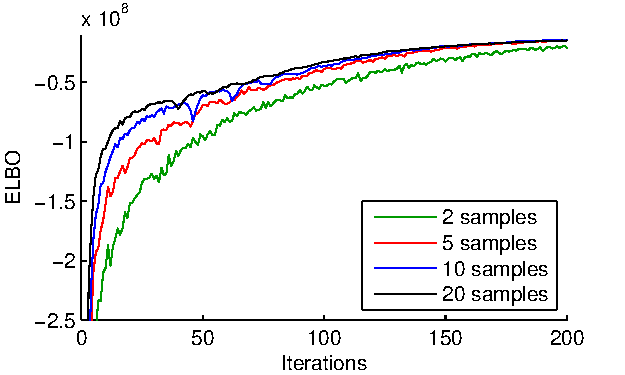
\includegraphics[width=0.36\textwidth]{figures/faces_nsamples_elbo.pdf}} \qquad
  \subfloat[Average variance.]{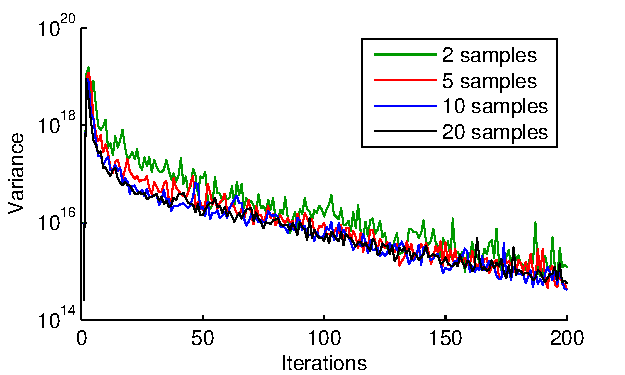
\includegraphics[width=0.36\textwidth]{figures/faces_nsamples_var.pdf}}
  \caption{Performance of \acrshort{G-REP} for different number of Monte Carlo samples.\label{fig:nsamples}}
\end{figure}



\subsection{Reconstructed images}

Here, we show some reconstructed observations for the three datasets involving images, namely, the binarized \textsc{mnist}, the Olivetti dataset, and Omniglot. We plot the reconstructed images as follows: we first draw one sample from the variational posterior, and then we compute the \emph{mean} of the observations for that particular sample of latent variables.

Figure~\ref{fig:images_faces} shows the results for the Olivetti dataset. The true observations are shown in the left panel, whereas the corresponding reconstructed images are shown in the center panel (for \acrshort{G-REP}) and the right panel (for \acrshort{ADVI}). We can observe that the images obtained from \acrshort{G-REP} are more detailed (e.g., we can distinguish the glasses, mustache, or facial expressions) than the images obtained from \acrshort{ADVI}. We argue that this effect is due to the variational family used by \gls{ADVI}, which cannot capture well sparse posterior distributions, for which samples close to $0$ are common.

This behavior is similar in the case of the digits from \textsc{mnist} or the characters from Omniglot. We show these images in Figures~\ref{fig:images_bmnist} and \ref{fig:images_omniglot}, respectively. Once again, images sampled from the \acrshort{G-REP} posterior are visually closer to the ground truth that images sampled from the \acrshort{ADVI} posterior, which tend to be more blurry, or even unrecognizable in a few cases.

\begin{figure}[ht]
  \centering
  \subfloat[True observations.]{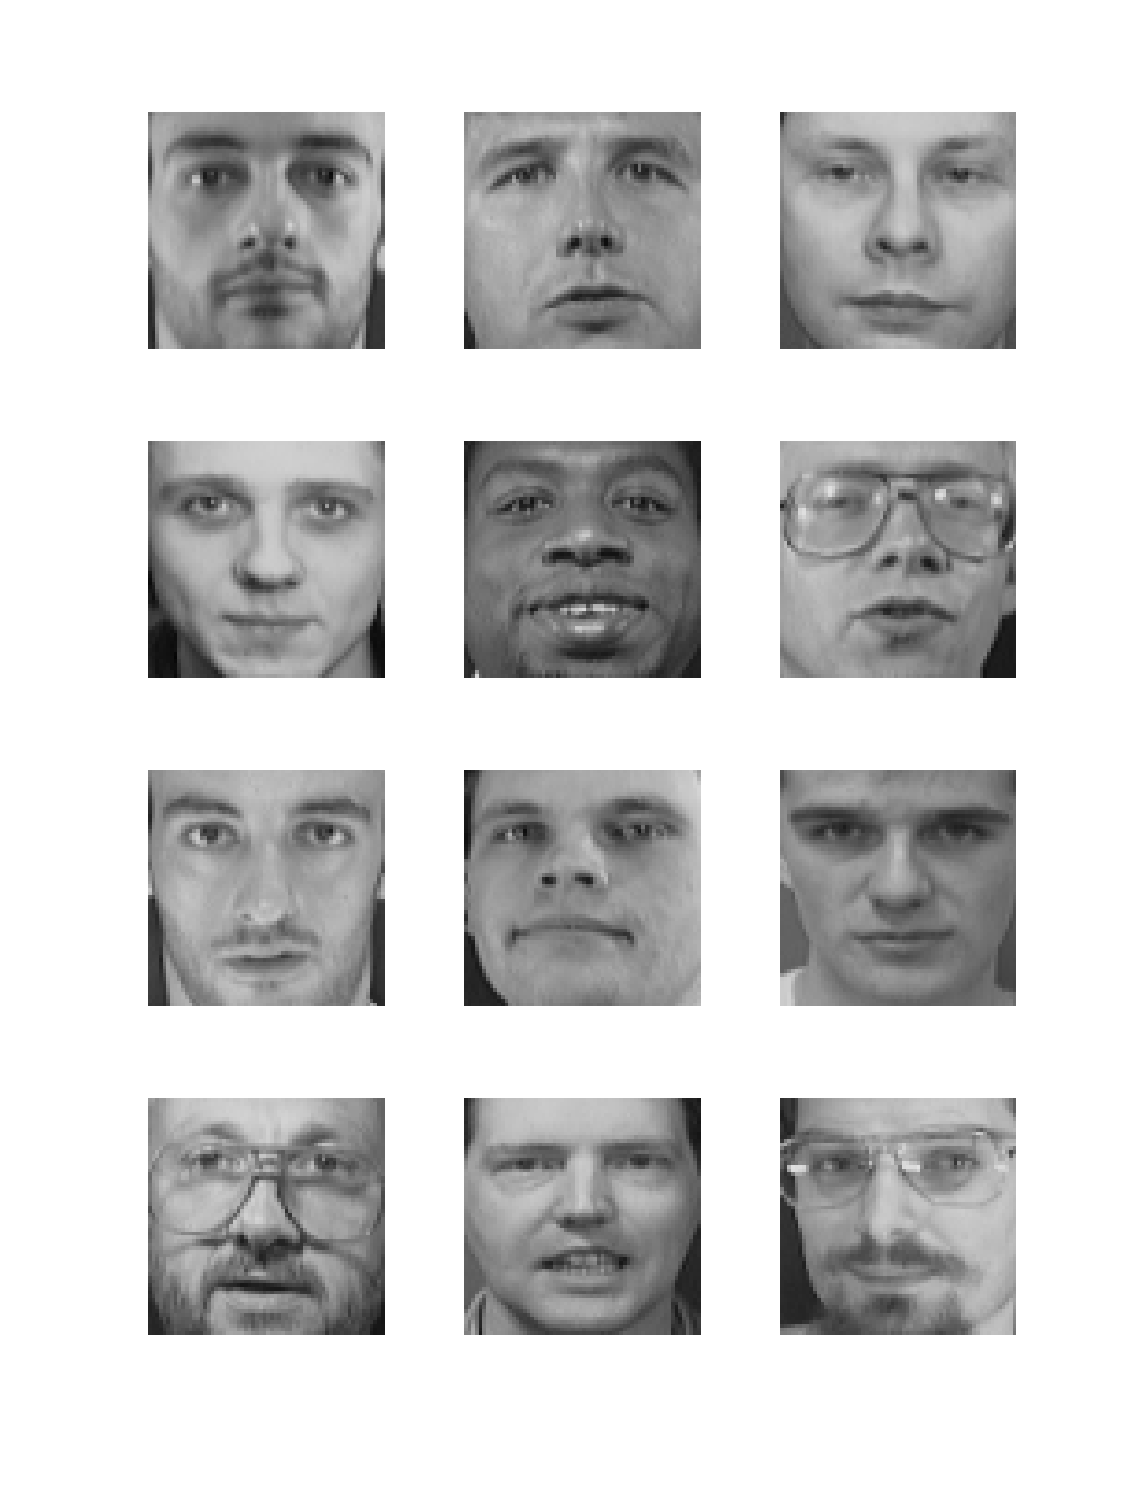
\includegraphics[width=0.33\textwidth]{figures/faces_true.pdf}}
  \subfloat[Reconstructed (\acrshort{G-REP}).]{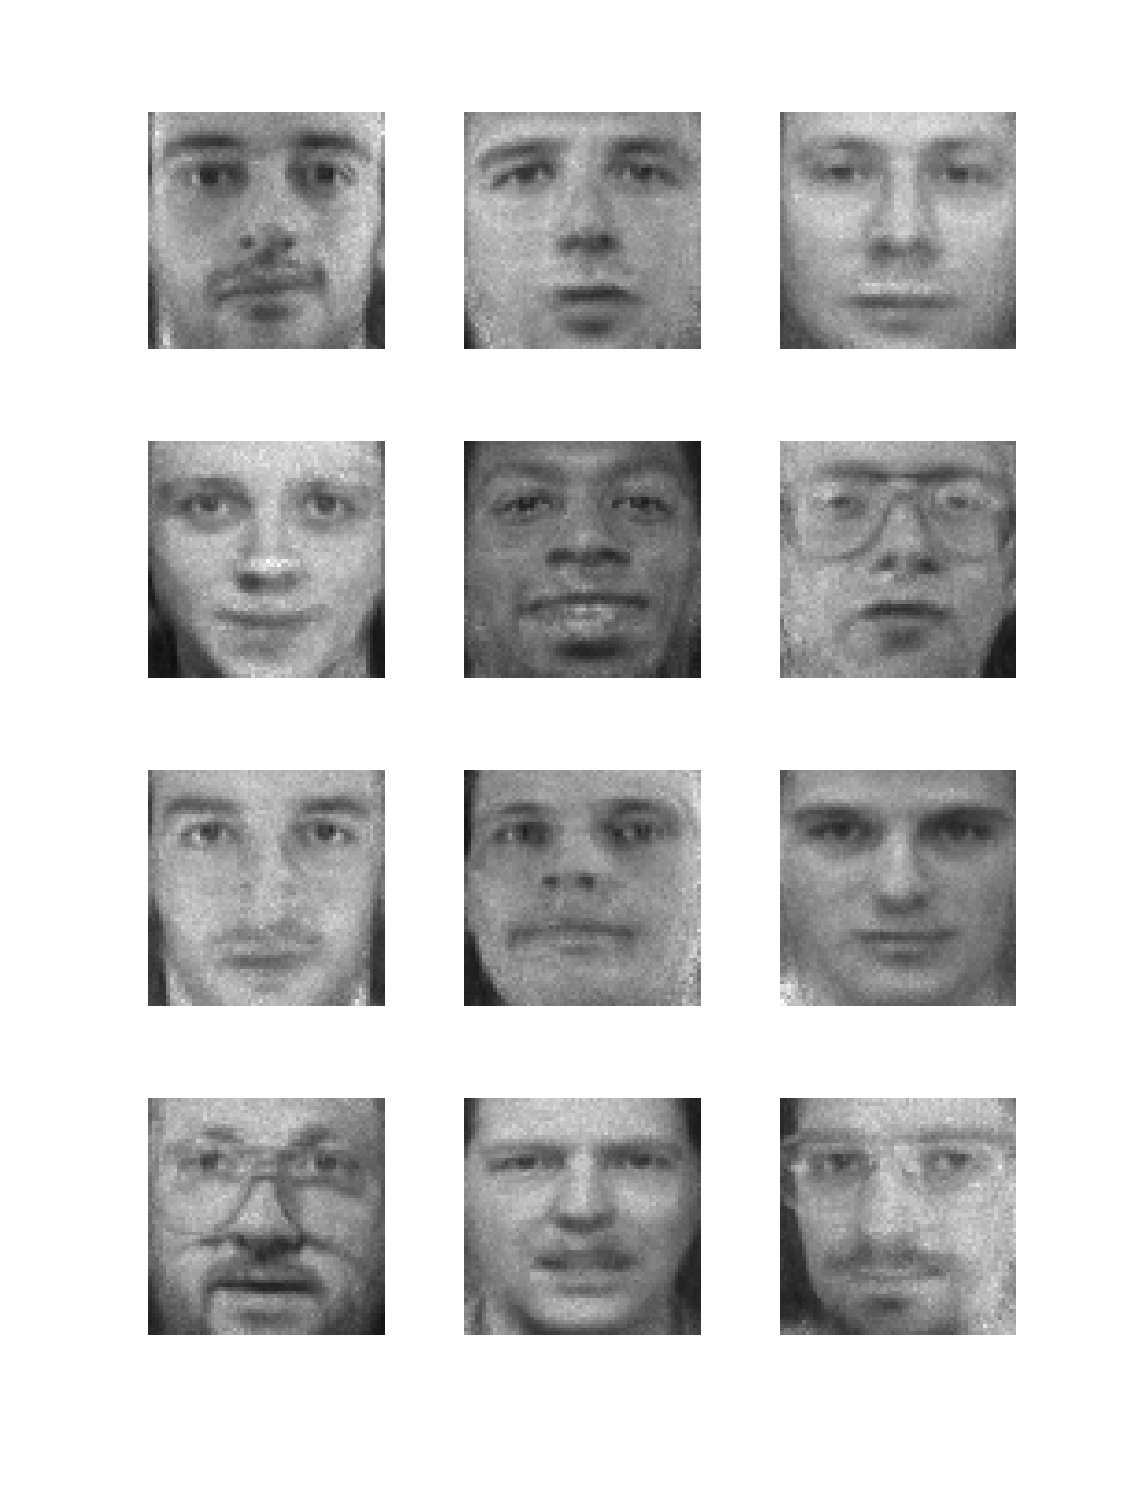
\includegraphics[width=0.33\textwidth]{figures/faces_our.pdf}}
  \subfloat[Reconstructed (\acrshort{ADVI}).]{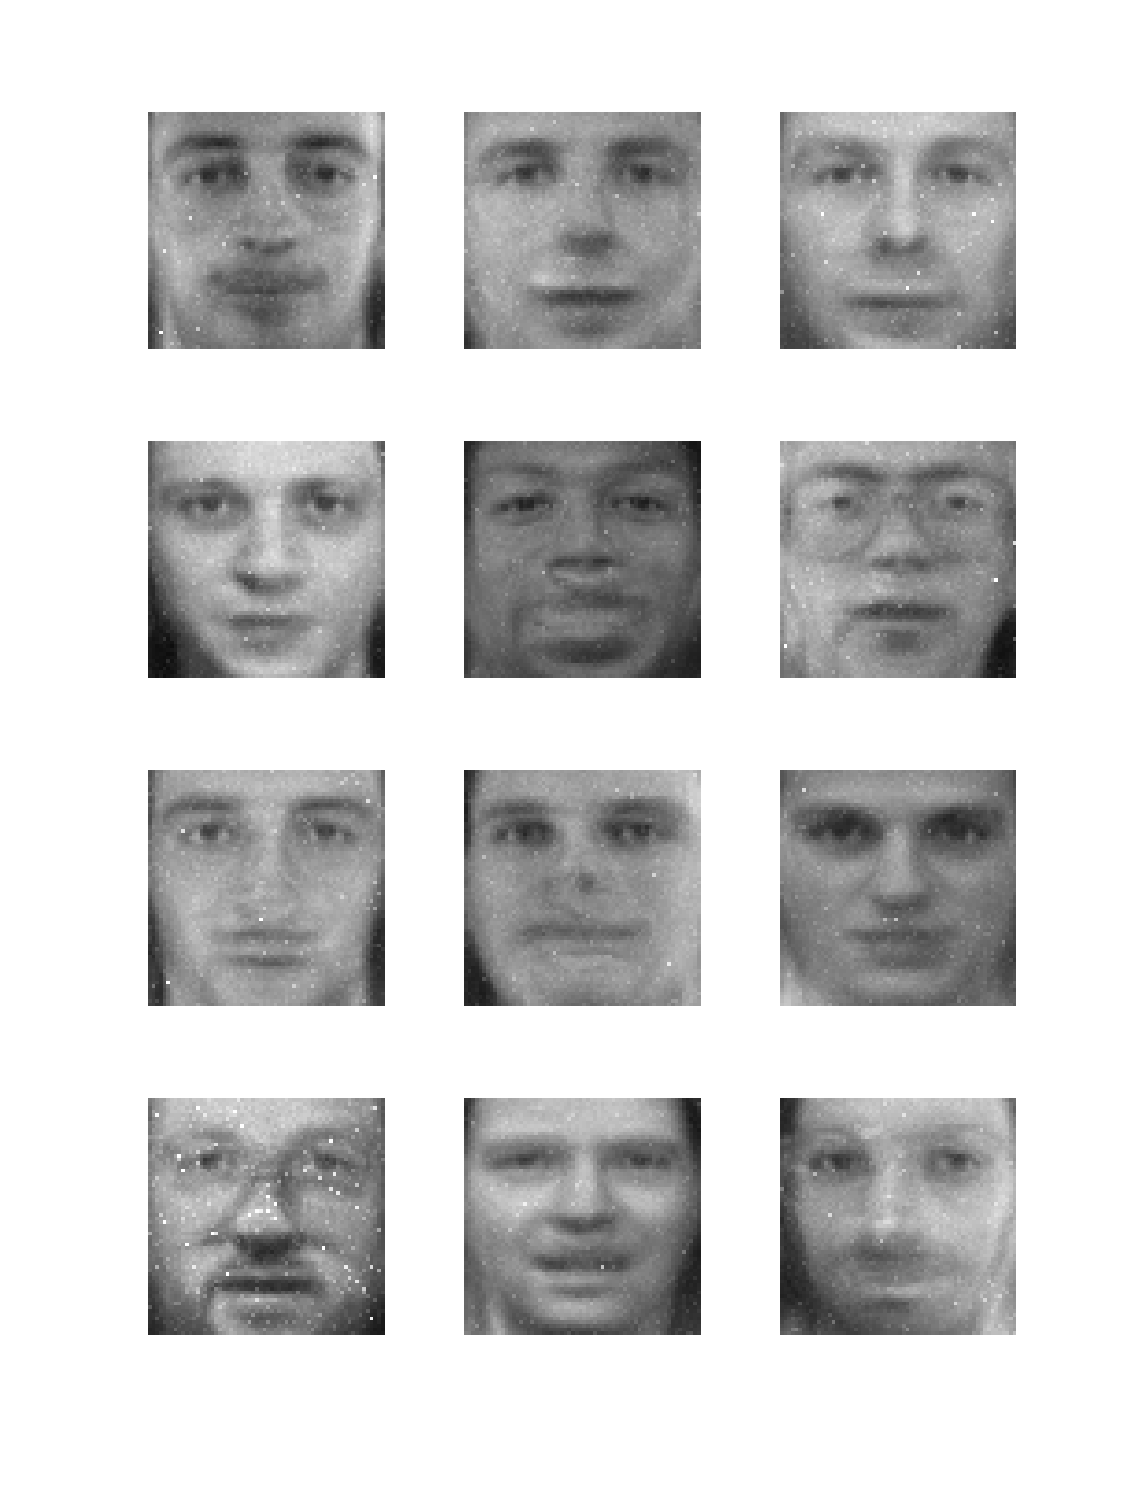
\includegraphics[width=0.33\textwidth]{figures/faces_advi.pdf}}
  \caption{Images from the Olivetti dataset. \gls{ADVI} provides less detailed images when compared to \acrshort{G-REP}.\label{fig:images_faces}}
\end{figure}

\begin{figure}[ht]
  \centering
  \subfloat[True observations.]{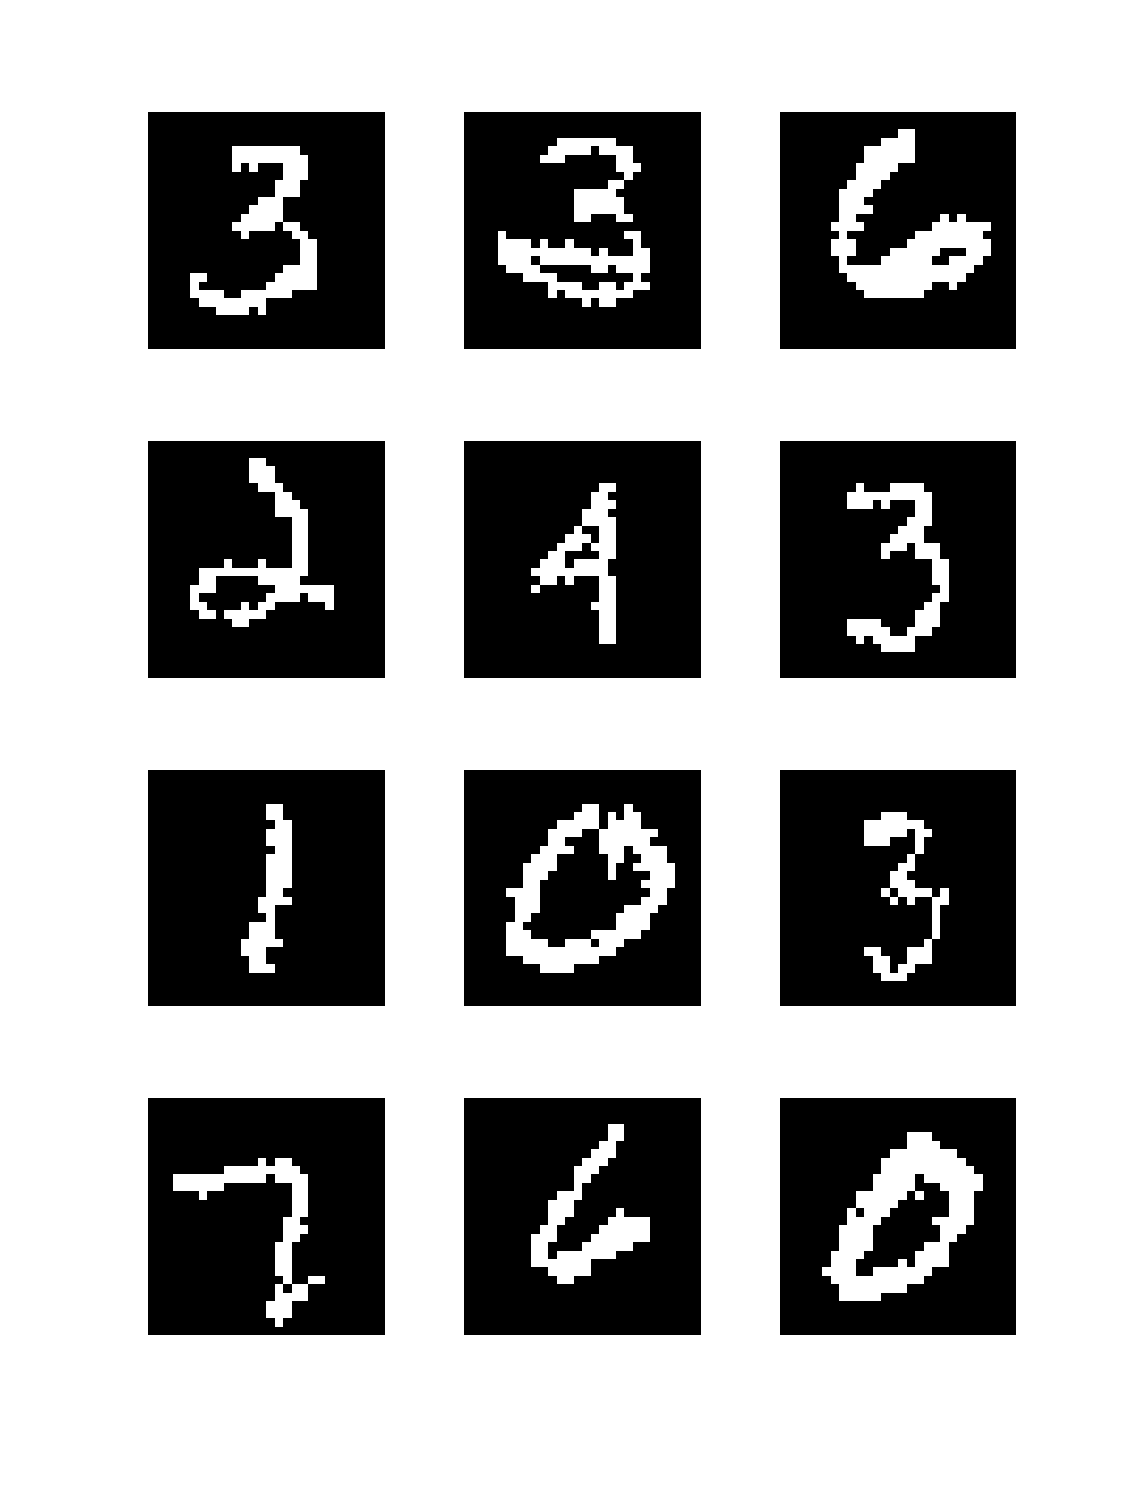
\includegraphics[width=0.33\textwidth]{figures/bmnist_true.pdf}}
  \subfloat[Reconstructed (\acrshort{G-REP}).]{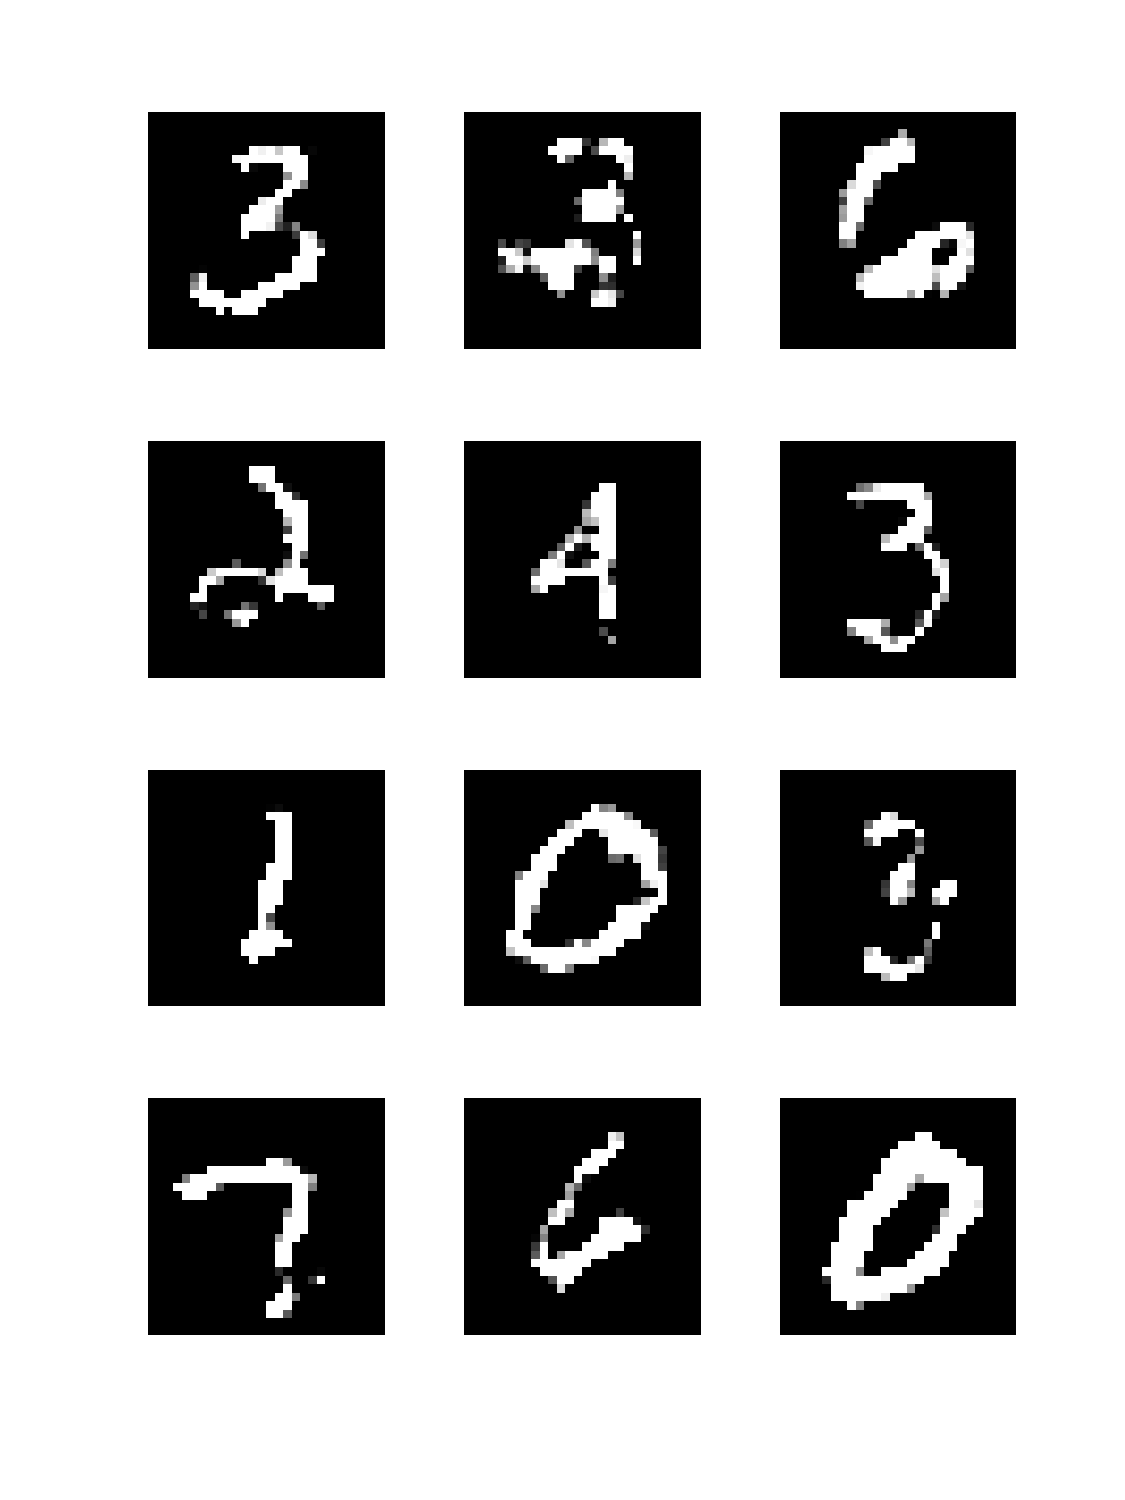
\includegraphics[width=0.33\textwidth]{figures/bmnist_our.pdf}}
  \subfloat[Reconstructed (\acrshort{ADVI}).]{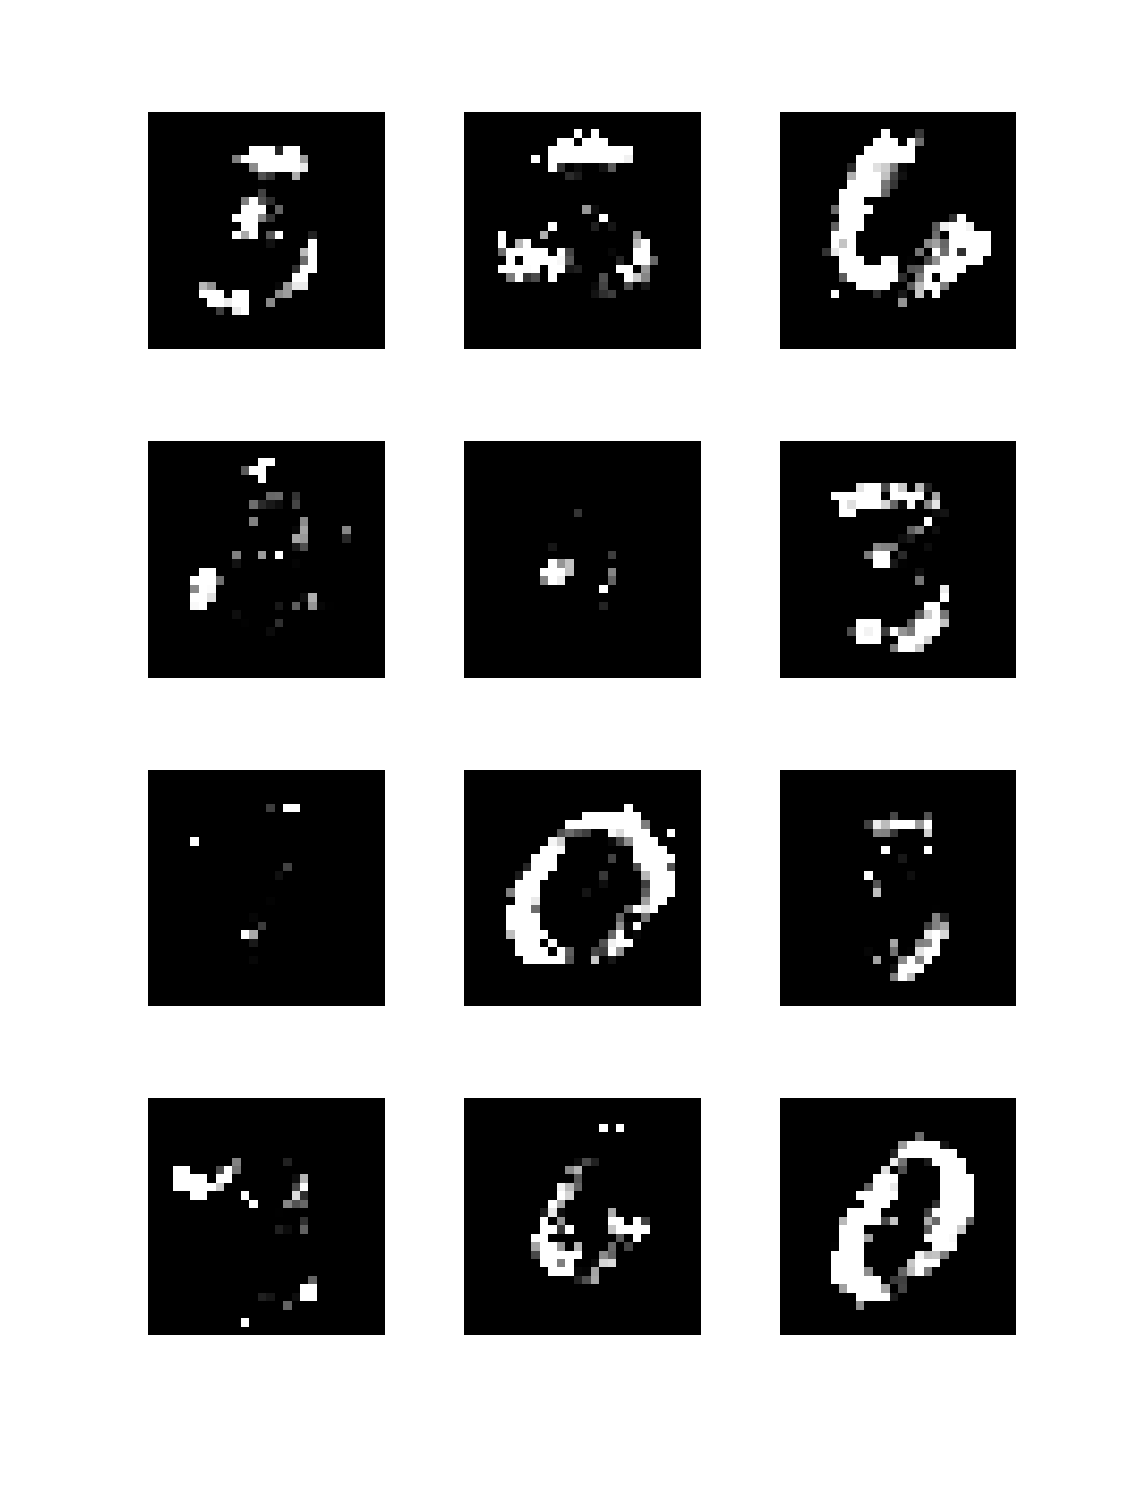
\includegraphics[width=0.33\textwidth]{figures/bmnist_advi.pdf}}
  \caption{Images from the binarized \textsc{mnist} dataset. \gls{ADVI} provides more blurry images when compared to \acrshort{G-REP}.\label{fig:images_bmnist}}
\end{figure}

\begin{figure}[ht]
  \centering
  \subfloat[True observations.]{
\includegraphics[width=0.33\textwidth]{figures/omniglot_true.pdf}}
  \subfloat[Reconstructed (\acrshort{G-REP}).]{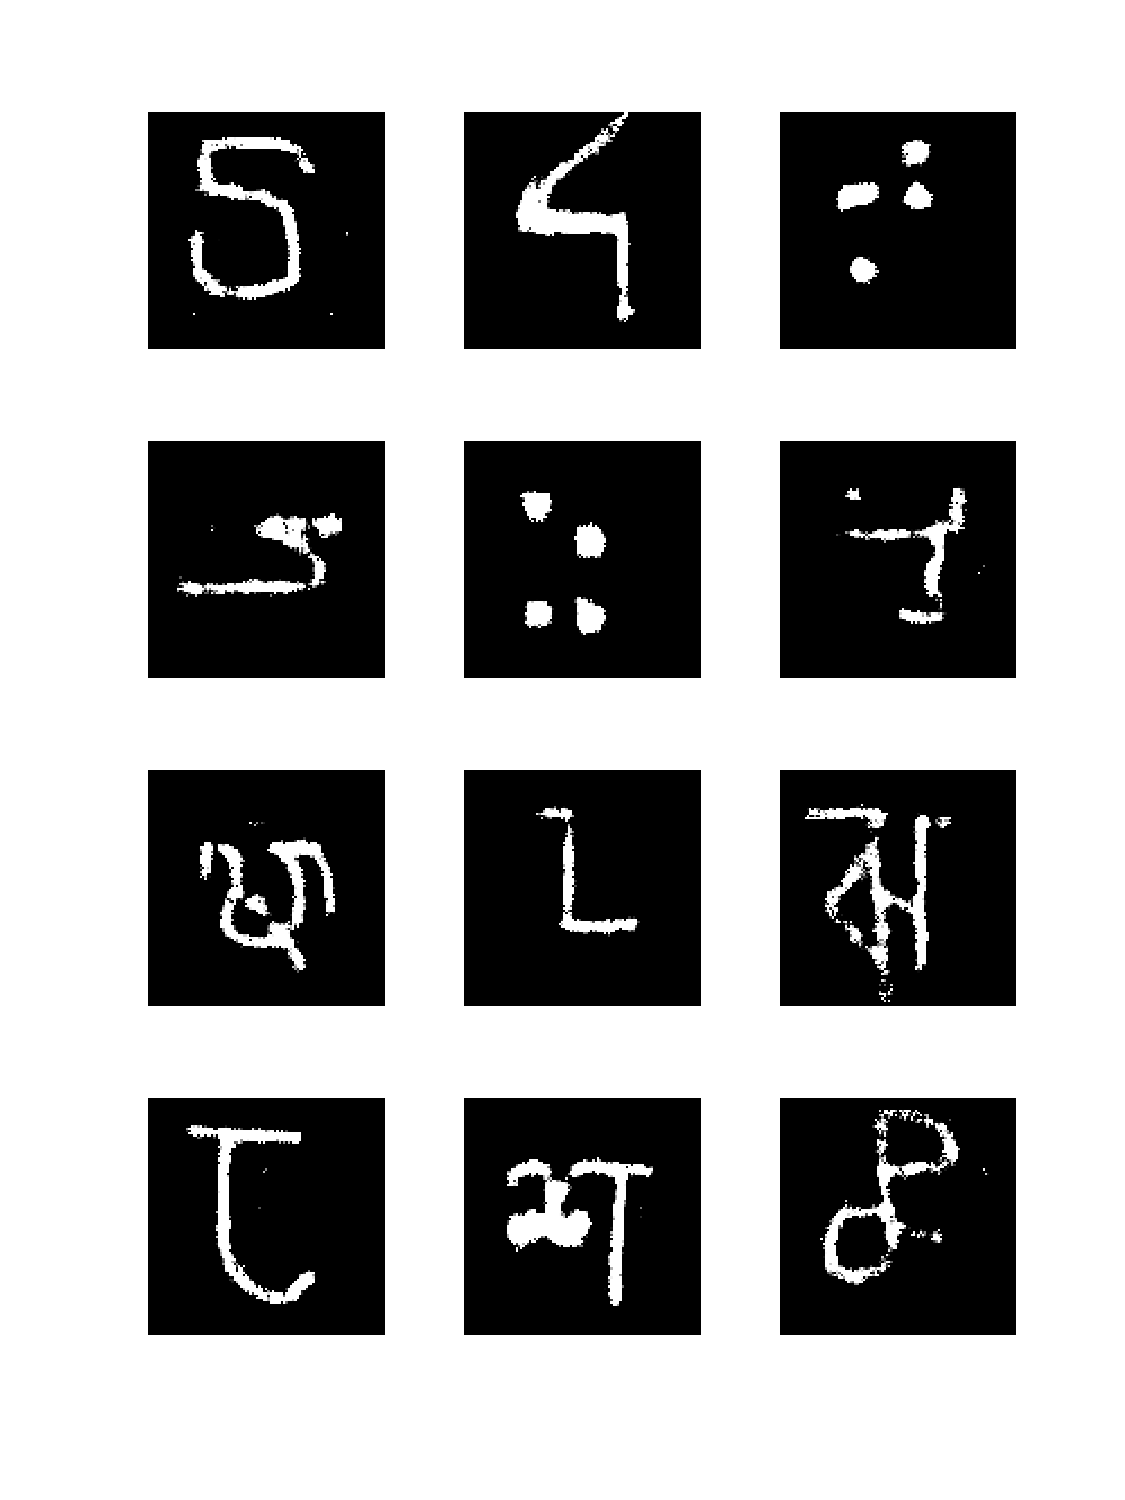
\includegraphics[width=0.33\textwidth]{figures/omniglot_our.pdf}}
  \subfloat[Reconstructed (\acrshort{ADVI}).]{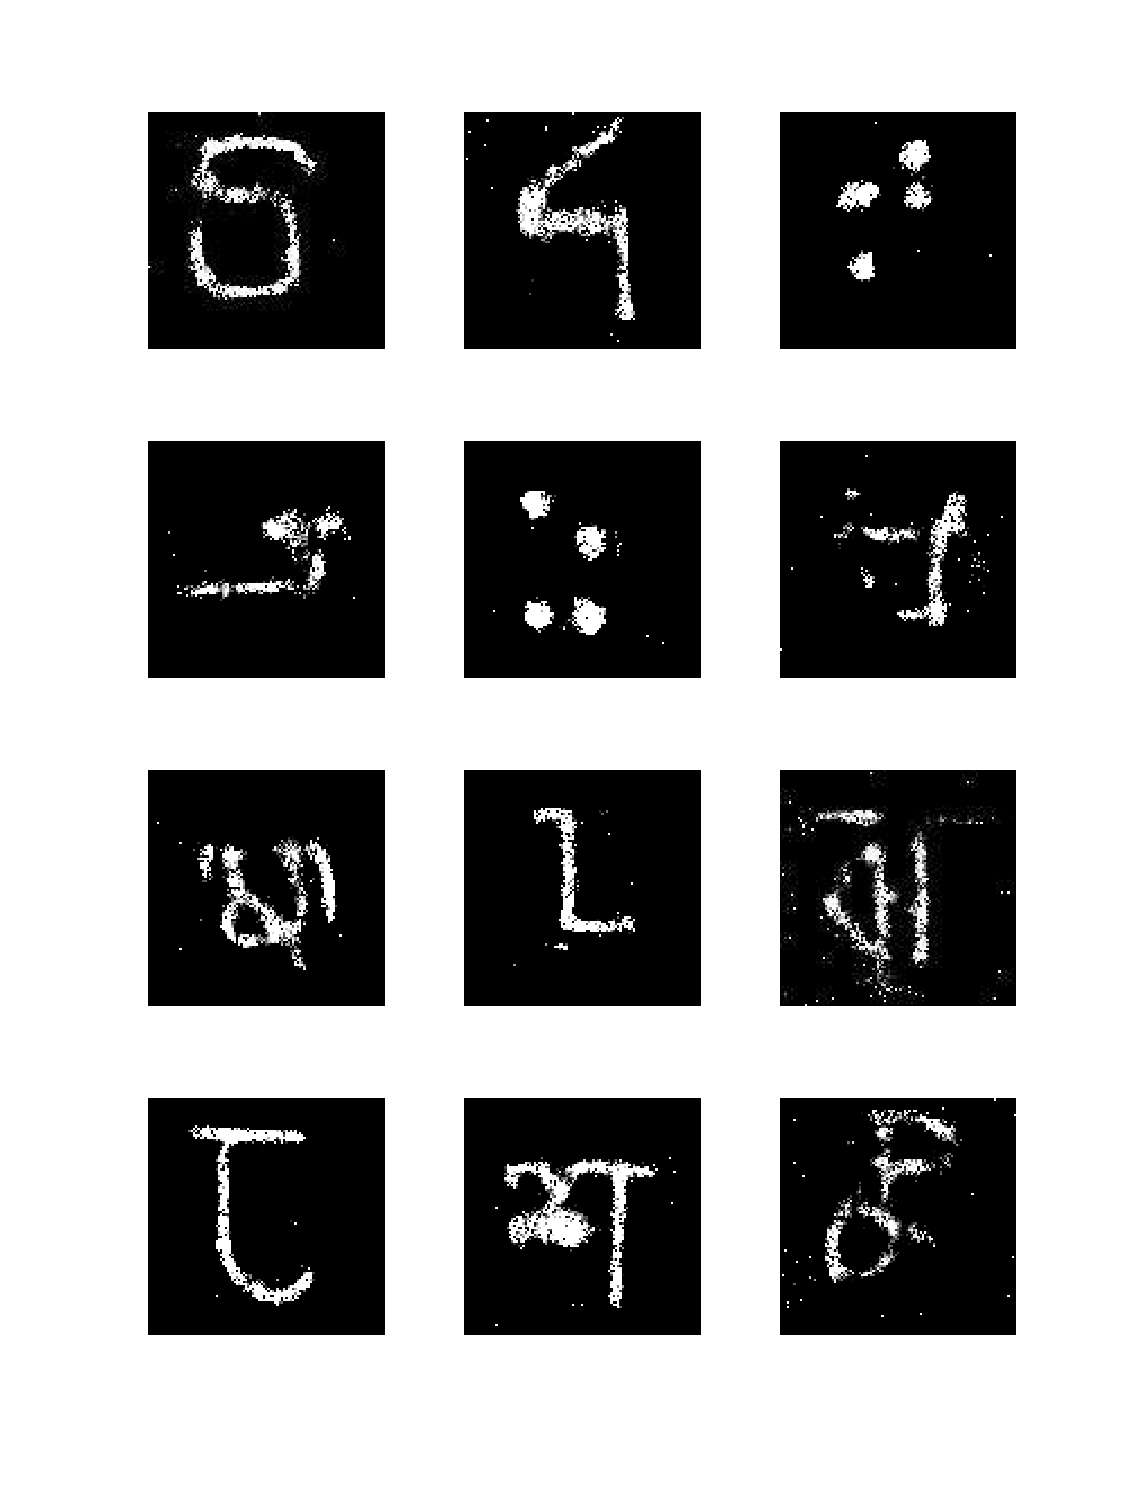
\includegraphics[width=0.33\textwidth]{figures/omniglot_advi.pdf}}
  \caption{Images from the Omniglot dataset. \gls{ADVI} provides more blurry images when compared to \acrshort{G-REP}.\label{fig:images_omniglot}}
\end{figure}





%%%%%%%%%%%%%%%%%%%%%%%%%%%%%%%%%%%%%%%%%%%%%%%%%%%%%%%%%%%%%%%%%
%\small
%\bibliographystyle{apa}
%\bibliography{/Users/franrruiz87/Dropbox/Research/fjrrLibrary}


\end{document}
